\documentclass[10pt,twocolumn]{article}
\usepackage[a4paper,margin=1.8cm,columnsep=0.7cm]{geometry}
\usepackage[T1]{fontenc}
\usepackage{newtxtext,newtxmath}
\usepackage{microtype}
\usepackage{graphicx}
\usepackage{booktabs}
\usepackage{amsmath}
\usepackage[numbers,sort&compress]{natbib}
\usepackage{xcolor}
\usepackage[hidelinks]{hyperref}
\usepackage{caption}
\captionsetup{font=small,labelfont=bf}
\setlength{\bibsep}{1pt}
\graphicspath{{figures/}}

\title{\Large\bfseries How Many Labels Does Eye-Contact Detection Need?\\
A Subject-Independent Comparison of Geometric Features,\\ Visual Foundation Models, and Gaze Estimators}
\author{FewGaze authors\\\small Code, configuration and all result files: \texttt{fewgaze} repository}
\date{}

\begin{document}
\maketitle

\begin{abstract}
\noindent
We measure how the number of labelled examples per class, $k$, affects classification of
\emph{camera-directed gaze} on people unseen during training. We use the Columbia Gaze Data Set:
5{,}878 images of 56 subjects after an audit removed one pair of duplicated images with conflicting
annotations. Every method keeps its backbone frozen and trains only a fixed logistic-regression head:
interpretable MediaPipe eye and head geometry, DINOv2-S embeddings, the L2CS-Net gaze estimator,
and CLIP. All methods share identical subject-disjoint folds, identical training selections
($k\in\{5,\dots,100,\text{ALL}\}$, five seeds) and a subject-level bootstrap.
Nine geometric features with a degree-2 logistic regression were best at every budget:
AUROC rose from $0.537$ at $k{=}5$ to $0.730$ at $k{=}100$ and $0.810$ with all training data.
A linear probe on DINOv2 stayed at chance ($\le0.513$). Post-hoc diagnostics show that its embeddings
encode head pose but not linearly decodable gaze.
L2CS-Net's zero-label angle-to-camera score reached $0.595$; a trained head on its two output angles
did not improve on it ($0.596$ at ALL). The task is hard: no method separated the 0° condition from the 5° neighbours
reliably. The analysis plan was committed before any experiment ran.
\end{abstract}

\section{Introduction}
Knowing whether someone looks at a camera is useful for video-mediated communication, social robots
and attentive interfaces. Detectors for eye contact in natural interaction exist~\cite{muller2018robust,zhang2017everyday},
but building one for a new setting starts with collecting labels, and the payoff of each label depends on the
representation it is spent on. Generic foundation models such as DINOv2~\cite{oquab2024dinov2} and
CLIP~\cite{radford2021clip} are often assumed to be sample-efficient. Gaze estimators such as
L2CS-Net~\cite{abdelrahman2023l2cs} encode gaze explicitly. Hand-crafted eye geometry is cheap and interpretable.
How these compare when labels are scarce, and when evaluation is on \emph{new people}, is rarely
measured directly.

We study a deliberately narrow question: \emph{for each representation, how does held-out-subject
performance grow with the number of labelled examples per class?} The target is \textbf{camera-directed
gaze under controlled capture}, a proxy for eye contact and not interpersonal eye contact itself.
Our contributions are:
(i)~a leakage-tested, subject-independent label-budget protocol in which every method shares folds,
training samples and test images, with the plan committed before the first run;
(ii)~learning curves, a simulated label-noise study and a head-pose analysis for four frozen representation families;
(iii)~diagnostics that explain the failure of generic embeddings.

\section{Related work}
Smith et al.~\cite{smith2013gazelocking} introduced \emph{gaze locking} and the Columbia Gaze Data Set,
detecting camera-directed gaze from rectified eye patches with PCA, MDA and an SVM.
Zhang et al.~\cite{zhang2017everyday} detect eye contact with arbitrary targets by discovering
gaze targets without supervision. Müller et al.~\cite{muller2018robust} combine gaze and speaking
behaviour for eye contact in multi-person conversations. Unlike these works, we do not propose a
detector; we measure sample efficiency under a shared protocol.
Appearance-based gaze estimation has advanced through large datasets such as
MPIIGaze~\cite{zhang2015mpiigaze,zhang2019mpiigaze}, Gaze360~\cite{kellnhofer2019gaze360} and
ETH-XGaze~\cite{zhang2020ethxgaze}; Cheng et al.~\cite{cheng2024survey} survey the area.
L2CS-Net~\cite{abdelrahman2023l2cs} regresses pitch and yaw with per-angle binned classification.
For geometry we use MediaPipe~\cite{lugaresi2019mediapipe} face-mesh and iris
landmarks~\cite{kartynnik2019facemesh,ablavatski2020iris}.

\section{Data and protocol}
\paragraph{Dataset and label.}
In Columbia Gaze~\cite{smith2013gazelocking}, 56 subjects sat in a chin rest at 2\,m while
a camera moved to five positions, giving head poses of $0^\circ,\pm15^\circ,\pm30^\circ$ relative to the camera.
At each position, subjects fixated a $7\times3$ grid of targets defined relative to that camera
($H\in\{0,\pm5,\pm10,\pm15\}^\circ$, $V\in\{0,\pm10\}^\circ$). Positives are $H{=}V{=}0$,
which the authors call gaze locking; all other cells are negatives, as in~\cite{smith2013gazelocking}.
Our audit (\texttt{audit\_dataset.py}) confirmed 5{,}880 readable $5184{\times}3456$ JPEGs and a complete
$56\times5\times21$ grid. It also found one byte-identical pair annotated with different horizontal gaze
($-15$P$-10$V, $H{=}0$ vs.\ $5$, subject 0007); both were excluded before modelling.
This leaves 280 positives and 5{,}598 negatives, a ratio of 1\,:\,20. The paper does not specify sign conventions;
the binary label does not depend on them.

\paragraph{Splits and budgets.}
Subjects were dealt into five folds with a fixed seed (11--12 test subjects per fold). Automated
tests verify subject-disjointness, full coverage and determinism. In each fold and for each seed
$s\in\{0..4\}$, one permutation per class of the training subjects' images is drawn, and the first $k$
are used. Budgets are therefore nested, and \textbf{every method receives the same samples}.
ALL means every training-subject image (about 225 positives and 4{,}480 negatives).

\paragraph{Representations (all frozen).}
\emph{Geometry}: MediaPipe Face Landmarker (478 points) on the image downscaled to 1600\,px. For each eye
we compute the iris-centre offset along and across the corner-to-corner axis and the lid aperture,
each divided by eye width; we add three head-rotation angles from MediaPipe's face transform, for nine features.
\emph{DINOv2-S}~\cite{oquab2024dinov2}: the CLS token of the 448\,px MediaPipe face crop resized to $224^2$.
\emph{L2CS-Net}~\cite{abdelrahman2023l2cs} (ResNet-50, Gaze360 weights): (pitch, yaw) from the $448^2$ crop.
We also use a \emph{zero-label} score: minus the angle between the predicted gaze and the camera axis.
\emph{CLIP} ViT-B/32~\cite{radford2021clip}: zero-shot softmax over two prompts fixed in advance
(``A photograph of a person looking directly toward / away from the camera.'').
MediaPipe found a face in all 5{,}878 images, so every method sees the same images.

\paragraph{Classifier, metrics, uncertainty.}
Logistic regression (C$=$1, balanced class weights, threshold 0.5) inside a scikit-learn~\cite{pedregosa2011sklearn}
pipeline fit on the training selection only. Hyperparameters were not tuned.
The positive class lies at the \emph{centre} of gaze space, and no linear function of a monotone
gaze proxy can isolate a centre. We therefore prespecified a degree-2 polynomial expansion for the
low-dimensional geometry and L2CS features. Embeddings receive a standard linear probe.
AUROC (primary) and balanced accuracy are averaged over the 25 fold$\times$seed runs.
95\% CIs come from a fold-stratified \emph{subject} cluster bootstrap with 1{,}000 replicates and
identical resamples for all methods, so differences are paired. The interval reflects which subjects
were tested, not retraining variability.

\begin{figure}[t]
\centering
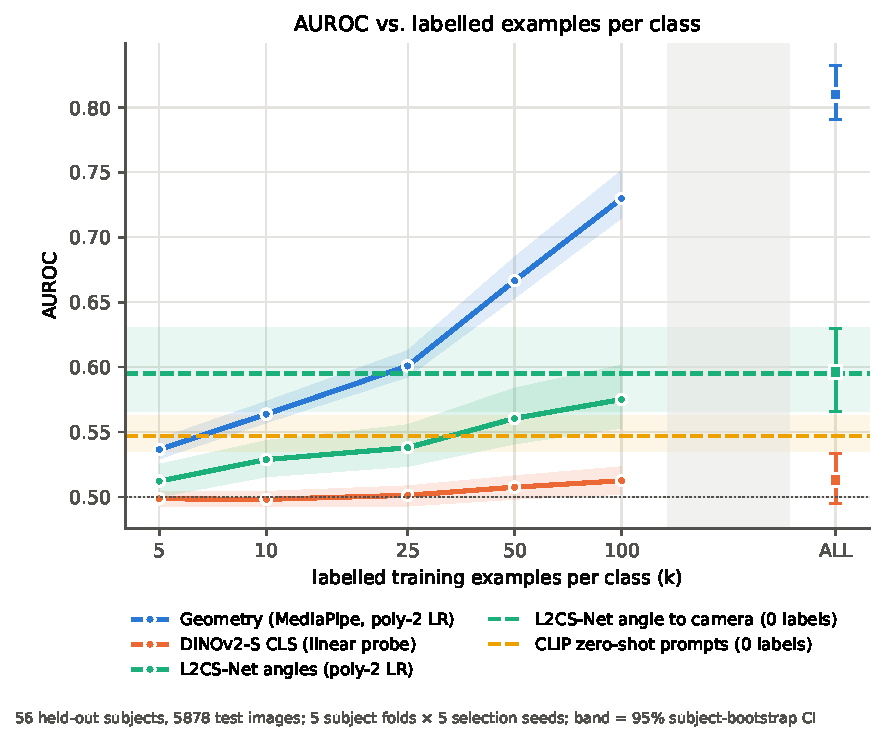
\includegraphics[width=\columnwidth]{fig3_learning_curves_auroc.pdf}
\caption{AUROC on held-out subjects vs.\ labelled examples per class (log scale). Bands: 95\% subject-bootstrap CIs;
dashed: methods that use no FewGaze labels. ALL (about 225 positives and 4{,}480 negatives) is plotted separately.}
\label{fig:lc}
\end{figure}

\begin{table}[t]
\centering\scriptsize
\setlength{\tabcolsep}{3pt}
\begin{tabular}{lcccccc}
\toprule
Method & $k=5$ & $k=10$ & $k=25$ & $k=50$ & $k=100$ & ALL \\
\midrule
Geometry (MediaPipe, poly-2 LR) & 0.537 & 0.564 & 0.601 & 0.667 & 0.730 & 0.810 \\
DINOv2-S CLS (linear probe) & 0.499 & 0.498 & 0.501 & 0.507 & 0.512 & 0.513 \\
L2CS-Net angles (poly-2 LR) & 0.512 & 0.529 & 0.538 & 0.560 & 0.575 & 0.596 \\
\midrule
Geometry (linear LR) & 0.504 & 0.509 & 0.515 & 0.516 & 0.520 & 0.555 \\
DINOv2-S mean-patch (linear probe) & 0.499 & 0.500 & 0.502 & 0.510 & 0.521 & 0.545 \\
L2CS-Net 2048-d features (linear probe) & 0.513 & 0.530 & 0.562 & 0.590 & 0.615 & 0.633 \\
CLIP ViT-B/32 (linear probe) & 0.505 & 0.507 & 0.516 & 0.529 & 0.545 & 0.567 \\
\midrule
L2CS-Net angle to camera (0 labels) & \multicolumn{6}{c}{0.595 (no training labels)} \\
CLIP zero-shot prompts (0 labels) & \multicolumn{6}{c}{0.547 (no training labels)} \\
\bottomrule
\end{tabular}
\caption{Mean AUROC over 5 folds $\times$ 5 seeds (CIs in \texttt{learning\_curves.csv}).
Top: primary; middle: ablations; bottom: zero-label methods.}
\label{tab:auroc}
\end{table}

\section{Results}
\paragraph{Learning curves.}
Geometry improved steadily with labels and led at every budget (Fig.~\ref{fig:lc}, Tab.~\ref{tab:auroc}):
AUROC was $0.537$ [0.529, 0.545] at $k{=}5$, $0.601$ [0.592, 0.613] at $k{=}25$, $0.730$ [0.715, 0.751] at $k{=}100$
and $0.810$ [0.791, 0.833] at ALL. Balanced accuracy was $0.527$, $0.578$, $0.686$ and $0.733$.
All three prespecified paired differences excluded zero at every budget (Tab.~\ref{tab:paired}).
For L2CS$-$DINOv2 at $k{=}5$ the lower bound was only just above zero.
The DINOv2 linear probe stayed at chance across budgets ($0.499$--$0.513$).
L2CS angles with a trained head rose from $0.512$ to $0.596$, matching but not improving on the zero-label
L2CS score ($0.595$ [0.566, 0.630]). CLIP zero-shot reached $0.547$ [0.535, 0.563].
For reference, geometry needed between 10 and 25 labels per class to match the zero-label L2CS score.
\emph{Ablations}: without the polynomial, geometry stayed near chance ($0.504$--$0.555$), confirming the
centre-region argument. L2CS's 2048-d features with a linear probe ($0.633$ at ALL) beat its two angles.
Neither DINOv2 mean-patch tokens ($\le0.545$) nor a CLIP probe ($\le0.567$) approached geometry.

\begin{table}[t]
\centering\scriptsize
\setlength{\tabcolsep}{3pt}
\begin{tabular}{llccc}
\toprule
Comparison & $k$ & $\Delta$AUROC & 95\% CI & CI excludes 0 \\
\midrule
dinov2 $-$ geometry & 5 & -0.038 & [-0.049, -0.028] & yes \\
dinov2 $-$ geometry & 25 & -0.100 & [-0.116, -0.089] & yes \\
dinov2 $-$ geometry & ALL & -0.297 & [-0.327, -0.270] & yes \\
l2cs $-$ geometry & 5 & -0.024 & [-0.039, -0.010] & yes \\
l2cs $-$ geometry & 25 & -0.063 & [-0.083, -0.045] & yes \\
l2cs $-$ geometry & ALL & -0.213 & [-0.246, -0.179] & yes \\
l2cs $-$ dinov2 & 5 & +0.014 & [+0.000, +0.028] & yes \\
l2cs $-$ dinov2 & 25 & +0.037 & [+0.021, +0.057] & yes \\
l2cs $-$ dinov2 & ALL & +0.083 & [+0.048, +0.117] & yes \\
\bottomrule
\end{tabular}
\caption{Prespecified paired comparisons ($\Delta$AUROC, identical bootstrap resamples). Shown for $k\in\{5,25,\text{ALL}\}$; all budgets in \texttt{paired\_differences.csv}.}
\label{tab:paired}
\end{table}

\paragraph{Where errors occur.}
At $k{=}25$, geometry labelled 71.8\% of true positives as camera-directed. It did so for 67.7\% of the
$|H|{=}5^\circ$ negatives, 50.8\% of the $|H|{\ge}10^\circ$ negatives and 43.2\% of the $V{=}\pm10^\circ$ negatives.
Its separation therefore comes almost entirely from the larger offsets. This is consistent with Smith et al.'s
estimate that their own detector tolerates about $\pm2.5^\circ$ horizontally~\cite{smith2013gazelocking}.
L2CS shows the same pattern (67.9\% of positives vs.\ 69.6\% of $|H|{=}5^\circ$ negatives).

\paragraph{Head pose.}
With all training data, geometry's AUROC was $0.891$ at a frontal pose. It fell to $0.835$/$0.847$ at
$\mp15^\circ$ and to $0.718$/$0.766$ at $\mp30^\circ$ (Fig.~\ref{fig:pose}; 56 positives per pose).
The other methods' pose profiles were flatter, with overlapping CIs, at a much lower overall level.

\begin{figure*}[t]
\centering
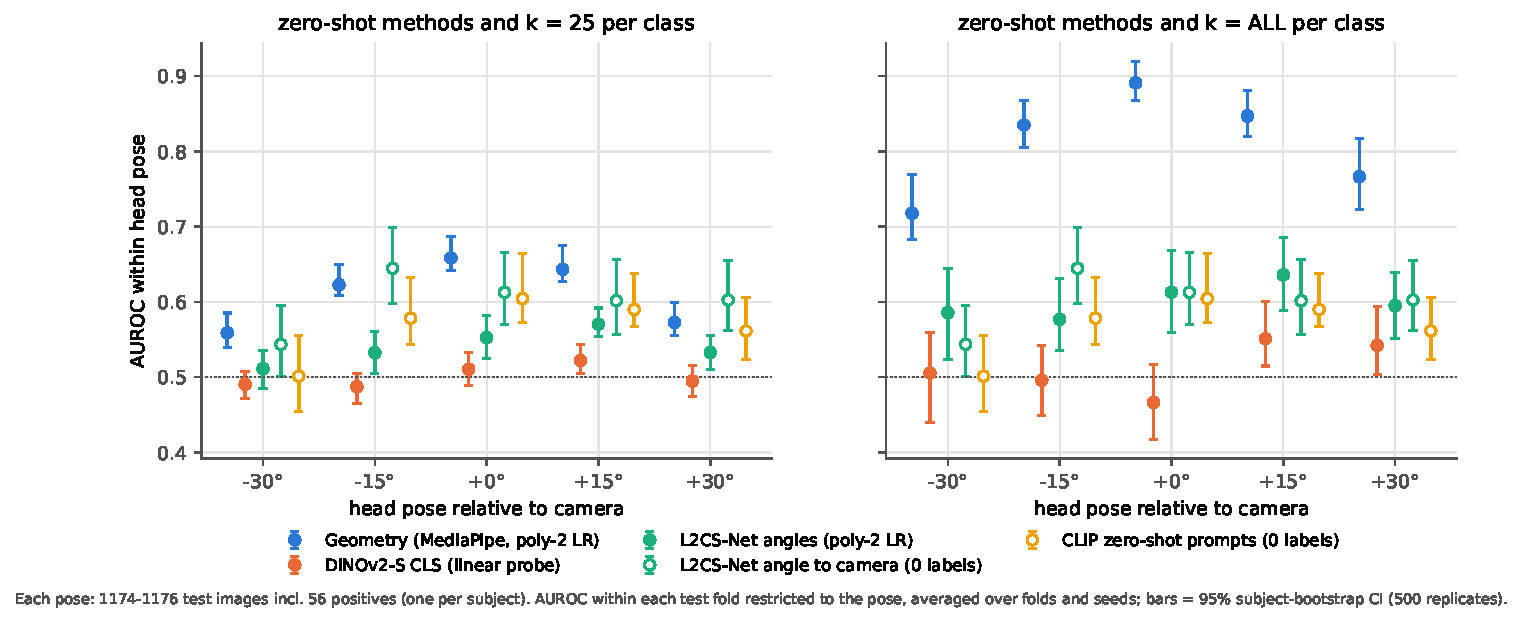
\includegraphics[width=0.8\textwidth]{fig6_head_pose.pdf}
\caption{AUROC within each head pose at $k{=}25$ and ALL (hollow markers: zero-label methods). 56 positives per pose; bars are 95\% subject-bootstrap CIs.}
\label{fig:pose}
\end{figure*}
\begin{figure*}[t]
\centering
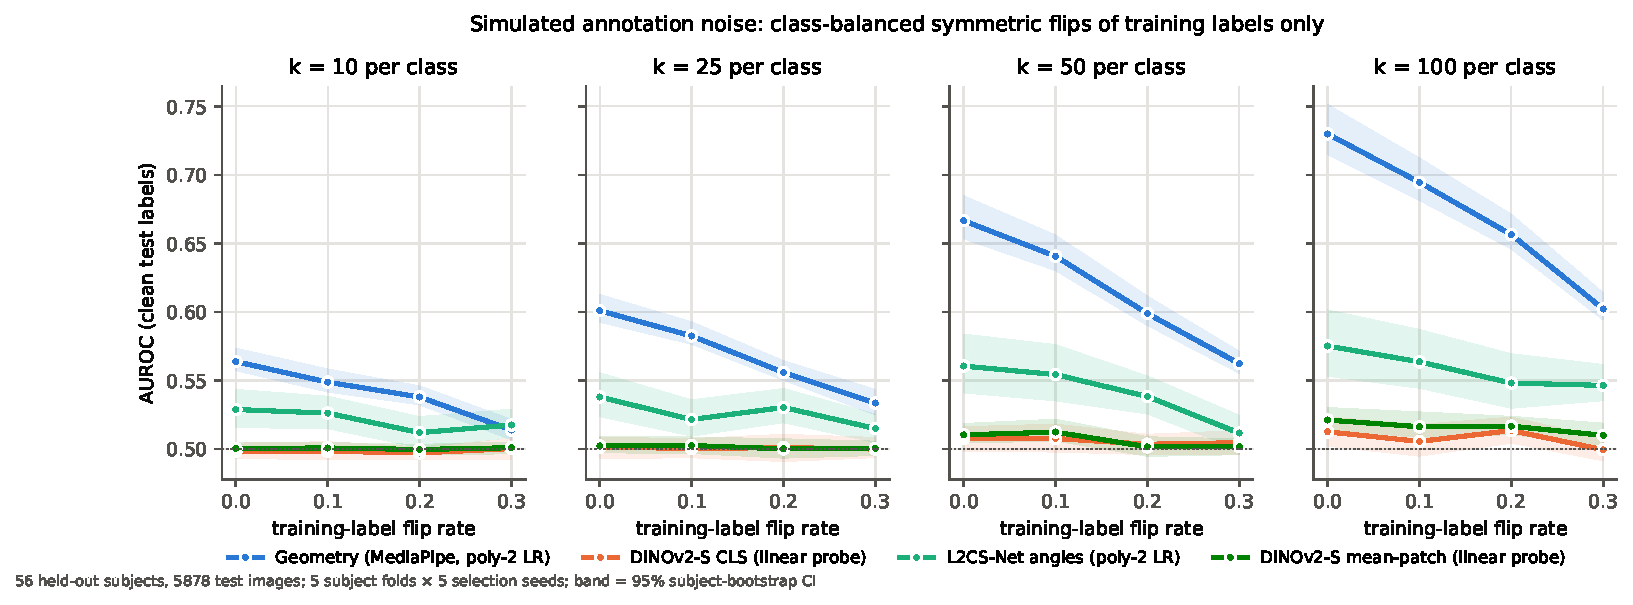
\includegraphics[width=0.92\textwidth]{fig5_label_noise.pdf}
\caption{Simulated label noise. Exactly the stated fraction of each class's training labels is flipped, with the same flips for all methods;
test labels stay clean. Bands: 95\% subject-bootstrap CIs.}
\label{fig:noise}
\end{figure*}

\paragraph{Label noise.}
Flipping training labels (Fig.~\ref{fig:noise}) degraded geometry roughly in proportion to the flip rate:
at $k{=}100$, AUROC fell from $0.730$ to $0.695$, $0.656$ and $0.602$ for 10/20/30\% flips.
At $k{=}25$, 10\% noise ($0.582$) cost less than reducing the clean budget to $k{=}10$ ($0.564$).
L2CS degraded less in absolute terms (from $0.575$ to $0.546$ at $k{=}100$), but from a much lower starting point.
DINOv2 stayed at chance throughout.

\paragraph{Post-hoc diagnostics (not prespecified).}
\emph{P1:} a subject-grouped ridge regression shows that DINOv2 CLS embeddings decode head pose almost perfectly
(held-out-subject $R^2{=}0.95$) but do not decode $H$ or $V$ ($R^2{<}0$). The geometry features decode
$H$ with $R^2{=}0.77$. The DINOv2 failure is therefore not a pipeline error: its global embedding of a
face crop is dominated by pose and identity. Consistent with this, its four most confident errors came from just two subjects.
\emph{P2:} feeding DINOv2 an eye-region crop instead raised AUROC at ALL from $0.513$ to $0.562$
($\Delta{=}{+}0.049$ [0.021, 0.082]). That is still far below geometry ($\Delta{=}{-}0.248$), so resolution
explains only part of the gap.

\paragraph{Cost.}
On an RTX~3050 laptop GPU, feature extraction took 35\,ms (DINOv2), 33\,ms (L2CS) and 18\,ms (CLIP) per image,
in addition to a shared 125\,ms CPU stage (JPEG decode, MediaPipe, cropping) that alone yields the geometry features.
Fitting any head took $\le$4\,s even at ALL.

\section{Discussion}
Under this protocol, the most sample-efficient representation was the simplest: nine geometric features, with
the right inductive bias for a centre-of-gaze-space target. Its curve was also the steepest, gaining
$0.19$ AUROC from $k{=}5$ to $k{=}100$. Generic self-supervised embeddings were not sample-efficient for this fine-grained,
identity-confounded distinction. Their invariance to small appearance changes is the wrong prior for detecting
a 5--10$^\circ$ eye rotation in an otherwise identical face.

The gaze estimator illustrates the role of prior knowledge. Without any FewGaze label, L2CS ranked images
better than any method trained on $k{\le}10$. Its learned head, however, gained nothing over the zero-label score.
On Columbia, L2CS predictions at the gaze-locked condition are biased (mean $\approx(-7^\circ,-6^\circ)$),
and per-subject zero-label AUROC ranged from $0.32$ to $0.94$. Its errors look like subject-specific
calibration offsets that a pooled two-feature classifier cannot remove. Its $k$ also undercounts its supervision,
since it was trained with gaze labels on Gaze360~\cite{kellnhofer2019gaze360}. The comparison is between
off-the-shelf systems, not architectures.

Even the best method did not resolve the dataset's hardest distinction, 0° vs.\ 5°. Absolute performance
(AUROC $\le0.81$) is far from deployable, and it should not be compared with the per-image accuracies reported by
Smith et al., who evaluated a different detector under a different protocol~\cite{smith2013gazelocking}.

\section{Limitations and ethics}
Results hold for one controlled dataset: 56 people, one lab, 2\,m distance, yaw-only head pose and a chin rest.
Camera-directed gaze in this setting is a proxy, not interpersonal eye contact.
Per-subject fixation accuracy is unknown, and the nearest negatives are only 5° away.
With 56 identities, CIs are subject-level approximations; they do not include retraining variance,
which we report separately as the SD across runs.
We kept prespecified settings, so other heads (e.g.\ non-linear probes on embeddings) might change
the ranking of the embedding methods; our P2 result suggests the input crop matters too.
The dataset has no per-subject demographic labels, so we make no fairness claims. Pretrained models carry the
biases of their training data. Gaze sensing can be misused for surveillance or attention scoring.
These classifiers are research artefacts and are unsuitable for monitoring or high-stakes use.

\section{Conclusion}
In a controlled, subject-independent setting, a handful of interpretable geometric features with a quadratic
decision boundary made the best use of labels, from 5 per class to several thousand. A frozen generic
embedding with a linear probe did not learn the task, and a pretrained gaze estimator mainly helped when no labels
were available. The main open question is whether per-subject calibration of gaze estimators, or local
eye-region representations, can resolve the last 5° that separates looking \emph{at} the camera from looking
just past it.

\paragraph{Reproducibility.}
The commands in the repository regenerate every number and figure. Images are not redistributed,
per the dataset's terms.

{\small
\bibliographystyle{abbrvnat}
\bibliography{references}
}
\end{document}
